% !TeX root = ../main.tex

\chapter{Experiments and Results}
\label{ch:experiments}

This chapter presents the experimental setup and results. Frozen-embedding baselines and a 500K architecture search establish the token-level pipeline. Data scaling then shows that, \emph{inside} the NT-v2 6-mer framework, volume dominates training tricks---and that the same volume does not raise a 13-mer ceiling. Depth-matched from-scratch controls and tokenization ablations separate pre-training from depth, and both from the tokenizer.

\section{Experimental Setup}
\label{sec:exp-setup}

\subsection{Dataset}

Training data is generated by simulating Illumina short reads (150~bp, HiSeq 2500 error profile) from the HGR-UMGS reference genome database~\cite{Almeida2019} using the ART read simulator~\cite{Huang2012}, following the same protocol as MetaTransformer~\cite{Wichmann2023}. The dataset covers:
\begin{itemize}
    \item \textbf{120 genera} and \textbf{1,535 species} of human gut microorganisms.
    \item \textbf{258M total reads} across all species.
    \item Highly skewed distribution: the most abundant genus (\textit{Collinsella}) accounts for 22.8\% of reads, while the rarest genera contribute $<$0.06\%.
\end{itemize}

We conduct experiments at three data scales by subsampling from the full dataset:
\begin{itemize}
    \item \textbf{500K} (imbalanced): The initial small-scale dataset preserving the natural class distribution. Train: 450K, validation: 50K.
    \item \textbf{5M} (balanced): Species-balanced subsample. Each of 1,535 species contributes $\sim$3,257 reads. Train: 4.5M, validation: 500K.
    \item \textbf{50M} (balanced): Species-balanced subsample. Each species contributes $\sim$32,573 reads. Train: 45M, validation: 5M.
\end{itemize}

\paragraph{Reads versus unique reads.} The read counts above (and the data-scaling axis in Figure~\ref{fig:data-scaling}) refer to \emph{training reads including duplicates}, which is the quantity the optimiser actually sees per epoch. The underlying source is heavily duplicated at the sequence level: the full read set contains 258.67M reads but only 42.64M \emph{unique} sequences ($6.07\times$ redundancy), a property of the source simulation rather than of our balancing. Consequently the larger balanced pools contain fewer distinct reads than their nominal size: the 50M pool comprises 17.76M unique reads and the 250M pool 41.94M unique reads---the latter already approaching the 42.64M source ceiling. This duplication structure is one reason data scaling saturates: beyond $\sim$50M reads, additional ``reads'' are increasingly repeats the model has already seen.

\subsection{Evaluation Protocol}

All models are evaluated on a held-out validation set using the metrics described in Section~\ref{sec:method-eval}. Unless otherwise noted, results are reported with RC TTA (Eq.~\ref{eq:rc-tta}). Depth-sweep and same-architecture tokenizer results in Sections~\ref{sec:exp-shallow} and~\ref{sec:exp-tokenization} use a shared \texttt{clean\_common} 100K file that is near-disjoint from the 50M training set (174 / 100{,}000 reads, 0.17\%, share a \texttt{seq\_id} with training). The original NT-Genus 67.07\% figure is the 50M internal-validation RC-TTA number; re-scoring that checkpoint on \texttt{clean\_common} gives 67.08\%.

\subsection{Hardware and Training Infrastructure}

All experiments are run on NVIDIA H100 80~GB HBM3 GPUs on the TWCC SLURM cluster. The 48-hour SLURM time limit requires checkpoint-resume support for training runs exceeding this duration.

\section{Phase 1: Frozen Embedding Baselines}
\label{sec:exp-frozen}

Before developing the token-level approach, we establish baseline performance using precomputed, mean-pooled embeddings from frozen GFMs.

\subsection{Setup}

Embeddings are extracted once from each of several pre-trained GFMs. A two-layer MLP classifier is trained on the resulting fixed-dimensional vectors. We evaluate models from two families:
\begin{itemize}
    \item \textbf{Evo-2 (7B params)}~\cite{Brixi2025}: A large-scale model based on the StripedHyena architecture. We extract embeddings from layer 2.
    \item \textbf{Nucleotide Transformer v2 (500M params)}: ESM-2-based model. We extract embeddings from the last hidden layer.
\end{itemize}

\subsection{Results}

\begin{table}[htbp]
    \centering
    \caption{Frozen embedding baselines for genus classification (120 classes, 500K dataset).}
    \label{tab:frozen-baselines}
    \begin{tabular}{lcc}
        \toprule
        \textbf{Method} & \textbf{Genus Accuracy} & \textbf{Notes} \\
        \midrule
        Uniform random ($1/K$) & 0.83\% & Lower bound \\
        Frequency baseline ($\sum p_k^2$) & 8.11\% & Predicting proportionally \\
        Majority class (always \textit{Collinsella}) & 22.84\% & Na\"ive baseline \\
        \midrule
        Evo-2 L2 mean-pool + MLP & 45.52\% & \\
        Evo-2 L2 + Focal Loss & 46.95\% & \\
        NT-v2 mean-pool + MLP & 51.70\% & Best frozen baseline \\
        NT-v2 mean-pool + MLP (RC-avg) & 51.70\% & With RC averaging \\
        \bottomrule
    \end{tabular}
\end{table}

The NT-v2 backbone consistently outperforms Evo-2 despite having 14$\times$ fewer parameters, suggesting that NT-v2's multi-species pre-training provides more suitable representations for metagenomic classification. NT-v2 achieves 51.70\% genus accuracy, which serves as our primary baseline.

\section{Phase 2: Token-Level Classification with LoRA}
\label{sec:exp-token-level}

We now present the token-level approach. Architecture and training-technique searches were run on 500K reads; they establish a plateau that motivates data scaling. The numbers that carry the argument of this chapter are at 5M and 50M.

\subsection{Architecture and Training Techniques (v1--v7, 500K Dataset)}
\label{sec:exp-techniques}

On 500K imbalanced reads, LoRA token-level training (v1) matches the frozen mean-pool baseline at 51.70\% genus accuracy. Reverse-complement augmentation (v3) reaches 53.92\% forward / 55.36\% RC TTA. Class-weighted cross-entropy with label smoothing (v2) collapses to 27.87\% ($-23.8$~pp), from the interaction of class weights and label smoothing on a 120-class imbalanced problem. Subsequent technique trials---shorter \texttt{max\_length} (v4), logit adjustment (v5/v5b), RC consistency (v6/v7)---remain in a $\pm0.5$~pp band around the v3 RC-TTA plateau (Table~\ref{tab:v4-v7}). Logit adjustment with $\tau=1.0$ is too aggressive (35.17\%); $\tau=0.3$ preserves micro accuracy while cutting F1$=$0 classes from 9 to 5. Combining RC consistency with logit adjustment (v6) is harmful; RC consistency alone (v7) is comparable to v3.

\begin{table}[htbp]
    \centering
    \caption{Architecture and training-technique experiments on the 500K dataset (genus classification). RC TTA results are shown where available. All technique variants after v3 stay within $\pm0.5$~pp of the v3 RC-TTA plateau except the failed logit-adjustment runs.}
    \label{tab:v4-v7}
    \small
    \setlength{\tabcolsep}{4pt}
    \begin{tabular}{llccccc}
        \toprule
        \textbf{Ver.} & \textbf{Description} & \textbf{Fwd Acc} & \textbf{RC TTA} & \textbf{F1-macro} & \textbf{F1$=$0} & \textbf{Gap} \\
        \midrule
        v1 & Token-level LoRA baseline & 51.70\% & --- & --- & --- & --- \\
        v2 & Class weights + LS (harmful) & 27.87\% & --- & --- & --- & --- \\
        v3 & RC aug, maxlen=128 & 53.92\% & 55.36\% & 25.82\% & 11 & 6.96\% \\
        v4 & maxlen=32 & 53.75\% & 55.29\% & 25.70\% & 9 & 6.25\% \\
        v5 & LA $\tau$=1.0 & 35.17\% & --- & --- & --- & --- \\
        v5b & LA $\tau$=0.3 & 52.29\% & 53.58\% & 26.53\% & 5 & --- \\
        v6 & RC consist.+LA & 35.87\% & 38.19\% & 22.88\% & --- & --- \\
        v7 & RC consist. only & 54.10\% & 55.18\% & 25.10\% & 11 & --- \\
        \bottomrule
    \end{tabular}
\end{table}

On v3, training accuracy continues to 62.7\% while validation saturates near 54\% (train--val gap $0\%\to 9\%$ by epoch 35). Figure~\ref{fig:training-dynamics} shows the same gap shrinking as data scale increases: severe overfitting at 500K, small gap at 5M, and well-generalised training at 50M.

\begin{figure}[htbp]
    \centering
    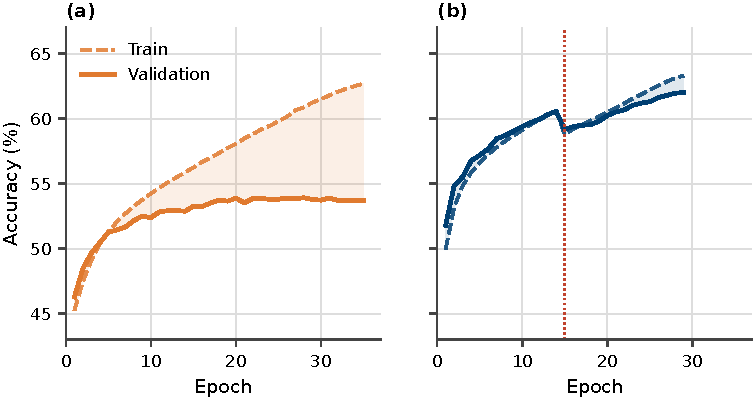
\includegraphics[width=\textwidth]{figures/training_dynamics.pdf}
    \caption{Training dynamics for v3 (500K, left), NT-Genus-5M (5M, centre), and NT-Genus (50M, right). Dashed lines show training accuracy; solid lines show validation accuracy. The shaded region highlights the train-validation gap. Dotted vertical lines mark learning-rate resets caused by SLURM timeout and job resumption; NT-Genus experienced two such resets (epochs 7 and 11) before the resume logic was corrected. Overfitting decreases systematically as data volume increases.}
    \label{fig:training-dynamics}
\end{figure}

\textbf{Conclusion}: All training techniques on the 500K dataset yield at most $\pm0.5$~pp improvement in RC TTA accuracy among the non-failed runs (range: 53.58\%--55.36\%). Inside this tokenizer and backbone, \emph{data volume}, not architecture or training tricks, is the bottleneck that the next section scales.

\section{Data Scaling Experiments}
\label{sec:exp-scaling}

Motivated by the accuracy plateau on 500K data and the comparison with MetaTransformer~\cite{Wichmann2023} (which trained on a large-scale balanced dataset trained on the full HGR-UMGS dataset of 2,505 species with coverage factor~4), we systematically scale training data.

\subsection{NT-Genus-5M: 5M Balanced Reads}

\subsubsection{Setup}

A 5M species-balanced subsample is drawn from the full 258M dataset. Each of 1,535 species contributes $\sim$3,257 reads, yielding near-perfect class balance. The v3 architecture and training configuration are retained (batch size 32, gradient accumulation 2, effective batch size 64), and training proceeds for 30 epochs.

Due to the 48-hour SLURM time limit, training required two jobs: the initial run completed 14 of 20 epochs before timeout, and a resumed run completed 16 additional epochs (epochs 15--30) using the \texttt{--resume} mechanism. A third job performed final evaluation.

\subsubsection{Results}

\begin{table}[htbp]
    \centering
    \caption{Genus classification results across data scales: v4 (500K), NT-Genus-5M (5M balanced), and NT-Genus (50M balanced).}
    \label{tab:v8-results}
    \small
    \setlength{\tabcolsep}{4pt}
    \begin{tabular}{lccccc}
        \toprule
        \textbf{Metric} & \textbf{v4 (500K)} & \textbf{NT-Genus-5M} & \textbf{$\Delta$\textsubscript{v4$\to$5M}} & \textbf{NT-Genus (50M)$^\dagger$} & \textbf{$\Delta$\textsubscript{5M$\to$50M}} \\
        \midrule
        Micro Accuracy (fwd)    & 53.75\% & 62.02\% & $+8.27$~pp & 66.29\%           & $+4.27$~pp \\
        Micro Accuracy (RC TTA) & 55.29\% & 63.05\% & $+7.76$~pp & \textbf{67.07\%}  & $+4.02$~pp \\
        Balanced Accuracy       & 25.23\% & 33.35\% & $+8.12$~pp & 39.91\%           & $+6.56$~pp \\
        F1 (weighted)           & 52.51\% & 61.06\% & $+8.55$~pp & 65.61\%           & $+4.55$~pp \\
        F1 (macro)              & 25.70\% & 37.97\% & $+12.27$~pp & \textbf{44.82\%} & $+6.85$~pp \\
        Top-3 Accuracy          & ---     & 81.70\% & ---        & 84.40\%           & $+2.70$~pp \\
        Top-5 Accuracy          & 82.91\% & 88.08\% & $+5.17$~pp & 90.03\%           & $+1.95$~pp \\
        Top-10 Accuracy         & 91.29\% & 94.23\% & $+2.94$~pp & 95.25\%           & $+1.02$~pp \\
        F1$=$0 classes          & 9       & 2       & $-7$       & \textbf{0}        & $-2$ \\
        Train-Val Gap           & 6.25\%  & 1.30\%  & $-4.95$~pp & $<$1\%            & --- \\
        \bottomrule
    \end{tabular}
    \begin{tablenotes}
        \small
        \item $\dagger$ NT-Genus final metrics (epoch~30, converged).
    \end{tablenotes}
\end{table}

The results reveal clear log-linear scaling behaviour:
\begin{enumerate}
    \item \textbf{Accuracy}: Each $10\times$ data increase yields a substantial but diminishing gain in RC TTA accuracy: $+7.76$~pp (500K$\to$5M) and $+4.02$~pp (5M$\to$50M). The sub-linear trend is consistent with logarithmic scaling laws.
    \item \textbf{Macro F1}: Data scaling disproportionately benefits rare classes: $+12.27$~pp at the first step and $+6.85$~pp at the second. At 50M reads, all 120 genera have non-zero F1 for the first time.
    \item \textbf{F1$=$0 classes}: The number of unclassifiable genera drops from 9 to 2 (NT-Genus-5M) and finally to 0 (NT-Genus), meaning every genus in the dataset is correctly predicted for at least some reads.
    \item \textbf{Overfitting}: The train-validation gap shrinks dramatically from 6.25\% (v4) to 1.30\% (NT-Genus-5M) to $<$1\% (NT-Genus), confirming that the model transitions from data starvation to well-generalised training as data volume increases.
\end{enumerate}

\subsubsection{Training Dynamics}

\begin{table}[htbp]
    \centering
    \caption{Training dynamics for NT-Genus-5M (5M balanced, 30 epochs). The gap between training and validation accuracy remains small throughout, in sharp contrast to the 500K experiments.}
    \label{tab:v8-dynamics}
    \begin{tabular}{ccccc}
        \toprule
        \textbf{Epoch} & \textbf{Train Acc} & \textbf{Val Acc} & \textbf{Train-Val Gap} & \textbf{Notes} \\
        \midrule
        1 & 49.96\% & 51.80\% & $-1.8$\% & \\
        5 & 55.97\% & 57.04\% & $-1.1$\% & \\
        10 & 58.93\% & 59.42\% & $-0.5$\% & \\
        14 & 60.60\% & 60.56\% & $+0.04$\% & 48h limit \\
        15 & 58.80\% & 59.18\% & $-0.4$\% & Resumed (LR reset) \\
        20 & 61.82\% & 60.59\% & $+1.2$\% & \\
        25 & 62.89\% & 61.77\% & $+1.1$\% & \\
        29$^\star$ & 63.32\% & 62.02\% & $+1.3$\% & Best epoch \\
        \bottomrule
    \end{tabular}
\end{table}

The temporary accuracy drop at epoch 15 is caused by the learning rate scheduler resetting to its warmup phase after resumption. The model recovers within 3--4 epochs and eventually surpasses the pre-interruption performance.

\subsection{NT-Genus Model: 50M Balanced Reads}
\label{sec:exp-v9}

Building on NT-Genus-5M, we scale training data by another $10\times$ to 50M balanced reads. The batch size is increased from 32 to 256 (with gradient accumulation reduced from 2 to 1, yielding an effective batch size of 256) to improve GPU utilization. The model is initialized from NT-Genus-5M's best checkpoint using \texttt{--init\_from} (transfer learning mode).

\begin{table}[htbp]
    \centering
    \caption{Configuration comparison between NT-Genus-5M and NT-Genus.}
    \label{tab:v9-config}
    \begin{tabular}{lcc}
        \toprule
        \textbf{Parameter} & \textbf{NT-Genus-5M} & \textbf{NT-Genus} \\
        \midrule
        Training reads & 4.5M & 45M \\
        Reads per species & $\sim$3,257 & $\sim$32,573 \\
        Batch size & 32 & 256 \\
        Gradient accumulation & 2 & 1 \\
        Effective batch size & 64 & 256 \\
        Epochs & 30 & 30 (converged) \\
        Weight initialization & Random & v8 best.pt \\
        Est.\ time per epoch & $\sim$3h & $\sim$5--6h \\
        \bottomrule
    \end{tabular}
\end{table}

\subsubsection{Results}

\begin{table}[htbp]
    \centering
    \caption{Comparison between NT-Genus-5M and NT-Genus (50M) for genus classification (120 classes).}
    \label{tab:v9-results}
    \begin{tabular}{lccr}
        \toprule
        \textbf{Metric} & \textbf{NT-Genus-5M} & \textbf{NT-Genus} & \textbf{$\Delta$} \\
        \midrule
        Micro Accuracy (fwd) & 62.02\% & \textbf{66.29\%} & $+4.27$~pp \\
        Micro Accuracy (RC TTA) & 63.05\% & \textbf{67.07\%} & $+4.02$~pp \\
        Balanced Accuracy & 33.35\% & 39.91\% & $+6.56$~pp \\
        F1 (weighted) & 61.06\% & 65.61\% & $+4.55$~pp \\
        F1 (macro) & 37.97\% & \textbf{44.82\%} & $+6.85$~pp \\
        Top-3 Accuracy & 81.70\% & 84.40\% & $+2.70$~pp \\
        Top-5 Accuracy & 88.08\% & 90.03\% & $+1.95$~pp \\
        Top-10 Accuracy & 94.23\% & 95.25\% & $+1.02$~pp \\
        F1$=$0 classes & 2 & \textbf{0} & $-2$ \\
        Best epoch & 29 & 30 (converged) & --- \\
        \bottomrule
    \end{tabular}
\end{table}

Scaling from 5M to 50M balanced reads yields a further $+4.02$~pp improvement in RC TTA accuracy (63.05\% $\to$ 67.07\%). Critically, the number of F1$=$0 classes drops to \textbf{zero}, indicating that all 120 genera are now correctly classified in at least some reads.

The marginal return diminishes relative to the previous $10\times$ scaling step: 500K$\to$5M yielded $+7.76$~pp while 5M$\to$50M yields $+4.02$~pp for the same multiplicative data increase, consistent with a logarithmic scaling relationship. This sub-linear trend is expected under log-linear scaling laws and suggests that continued data scaling alone will not close the remaining gap with MetaTransformer.

\paragraph{Training progress and LR restart incidents.}
NT-Genus training required multiple SLURM jobs due to the 48-hour time limit. Before a bug fix was applied to the checkpoint-resume logic, two job restarts inadvertently reset the cosine learning-rate scheduler to its initial warmup phase, causing temporary accuracy dips: $-0.54$~pp at epoch~7 and $-1.39$~pp at epoch~11. In both cases the model recovered within 3--5 epochs and surpassed the pre-dip performance level. The underlying issue---\texttt{EarlyStopping.best} being silently set to \texttt{None} from an incomplete checkpoint key---was corrected in the resume logic; from epoch~17 onward the scheduler state is correctly restored and the learning rate continues its cosine decay without interruption.

NT-Genus training completed at epoch~30 (April~2026), reaching a forward validation accuracy of \textbf{66.29\%} and RC~TTA accuracy of \textbf{67.07\%} (Figure~\ref{fig:learning-curves}). The learning curve plateaued between epochs~26 and~30 as the cosine schedule reached its minimum, indicating convergence.

\begin{figure}[htbp]
    \centering
    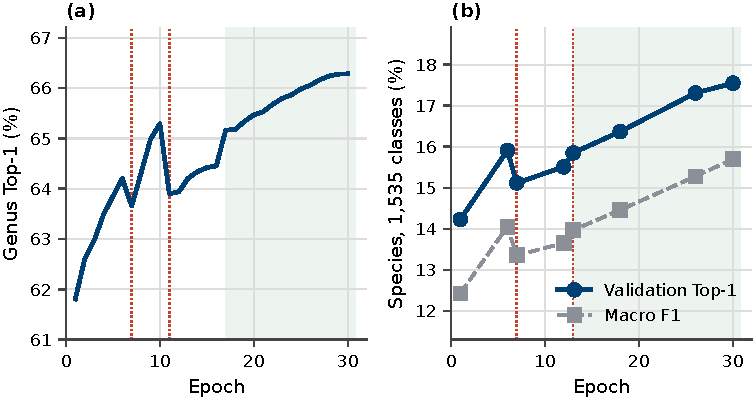
\includegraphics[width=0.95\textwidth]{figures/learning_curves.pdf}
    \caption{Full validation accuracy curves for NT-Genus (genus, left) and NT-Species (species, right) over all completed epochs. Red dotted vertical lines mark epochs where a SLURM job restart incorrectly reset the cosine LR scheduler, causing a temporary accuracy dip. The green shaded region indicates epochs trained after the resume bug fix was applied, during which the LR schedule correctly continues its cosine decay.}
    \label{fig:learning-curves}
\end{figure}

\subsection{Data Scaling Analysis}

\begin{table}[htbp]
    \centering
    \caption{Data scaling analysis: genus classification performance across data volumes. The 250M entry is the warm-started model (initialised from the 50M checkpoint and held out of the log-linear fit); the from-scratch 250M variant instead reaches 64.84\%. Only accuracy is reported for the 250M saturation experiment.}
    \label{tab:scaling}
    \begin{tabular}{rcccc}
        \toprule
        \textbf{Data Volume} & \textbf{RC TTA Acc} & \textbf{F1-macro} & \textbf{F1$=$0} & \textbf{Gap} \\
        \midrule
        500K (imbalanced) & 55.29\% & 25.70\% & 9 & 6.25\% \\
        5M (balanced) & 63.05\% & 37.97\% & 2 & 1.30\% \\
        50M (balanced) & \textbf{67.07\%} & \textbf{44.82\%} & \textbf{0} & $\sim$0.7\% \\
        250M (balanced, warm-start) & 67.29\% & --- & --- & --- \\
        MetaTransformer (HGR-UMGS full) & $\sim$98\% & --- & --- & --- \\
        \bottomrule
    \end{tabular}
\end{table}

The data scaling analysis reveals a clear relationship between training data volume and classification performance \emph{inside the NT-v2 6-mer framework}. The transition from 500K to 5M reads ($10\times$ increase) yields $+7.76$~pp in accuracy and $+12.27$~pp in macro F1. Meanwhile, all training technique ablations on the 500K dataset (v3--v7) produced at most $\pm0.5$~pp variation. Data volume, not architecture or training tricks, is therefore the primary determinant of 6-mer accuracy up to 50M. It is not the determinant of the residual gap to MetaTransformer: the 250M run below and Section~\ref{sec:exp-tokenization} show that gap is tokenizer-bound.

The published MetaTransformer genus recall of 98.3\% used a different data budget and tokenizer; it is not evidence that we simply need more 6-mer reads.

\figref{fig:data-scaling} plots genus RC TTA accuracy against training data volume on a logarithmic scale, with a log-linear fit to our three data points. The fitted curve projects that closing the gap with MetaTransformer would require training data well beyond our 50M-read scale, consistent with diminishing returns under logarithmic scaling.

\begin{figure}[htbp]
    \centering
    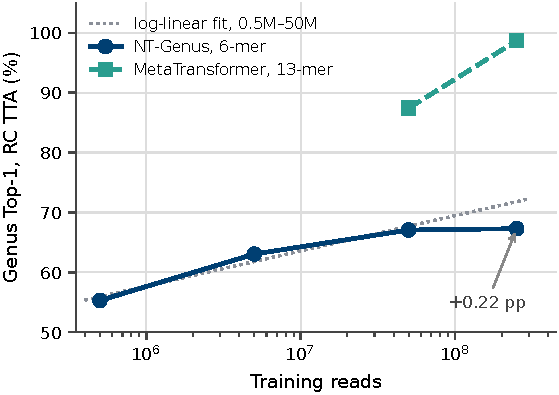
\includegraphics[width=0.80\textwidth]{figures/data_scaling.pdf}
    \caption{Genus RC TTA accuracy versus training data volume (log scale). The horizontal axis counts \emph{training reads including duplicates} (the per-epoch sample count); the corresponding \emph{unique}-read counts are smaller (50M$\to$17.8M, 250M$\to$41.9M unique, against a 42.6M source ceiling). Green circles mark our results at three data scales; the red star marks MetaTransformer's reported genus recall. The blue dashed line is a log-linear fit to our three data points. Per-$10\times$ accuracy gains diminish from $+7.76$~pp (500K$\to$5M) to $+4.02$~pp (5M$\to$50M). The fourth green circle (v15, 250M) continues the same warm-started series but is held out of the fit; at 67.29\% it falls well below the $\sim$71\% the log-linear fit would project at that scale---the trajectory flattens off its own projection, directly demonstrating that accuracy saturates beyond 50M rather than continuing along the trend. The MetaTransformer star marks reported genus recall (98.3\%); its x-position is based on training throughput (300K steps $\times$ batch~2,048) and is not directly comparable to our dataset-size axis.}
    \label{fig:data-scaling}
\end{figure}

\paragraph{Beyond 50M: the 6-mer model saturates, but the 13-mer model does not.}
The projection above tentatively attributes the residual gap to insufficient data. To test this directly, we scaled the balanced subsample by a further $5\times$ to 250M reads and trained two variants on a $64\times$H200 DDP cluster: a warm-started model initialised from the 50M NT-Genus checkpoint (mirroring the $5\text{M}\to 50\text{M}$ transfer) and a from-scratch model. Evaluated on an independent, read-disjoint test set under the identical RC-TTA protocol---on which the 50M NT-Genus model reproduces its $67.07\%$ to within $0.05$~pp---the 250M warm-started model attains only \textbf{67.29\%} genus Top-1 (RC~TTA), a $+0.22$~pp change over 50M despite the $5\times$ data increase, while the from-scratch 250M model is in fact lower at $64.84\%$. For the NT-v2 6-mer model, data scaling therefore \emph{saturates} beyond 50M rather than continuing along the log-linear trend.

Crucially, this saturation is a property of the \emph{tokenization}, not of the data or the single-genome-per-species reference. Trained on the \emph{same} reads, MetaTransformer with overlapping 13-mer tokenization continues to improve sharply with scale: on a common clean held-out pool its genus Top-1 rises from 87.5\% at 50M (the 87.42\% of Section~\ref{sec:exp-tokenization}) to \textbf{98.7\%} at 250M---and from 83.0\% to 98.5\% on a stricter ``leftover'' pool constructed to be sequence-ID-disjoint from both training sets, which rules out leakage. The identical $5\times$ data increase that moves the 6-mer model by $+0.22$~pp moves the 13-mer model by ${\sim}+11$~pp. The additional reads are therefore not redundant in any absolute sense: they carry discriminative signal that a non-overlapping 6-mer representation cannot resolve but an overlapping 13-mer one can. What saturates at 50M is the \emph{information ceiling of the 6-mer tokenizer}, not the data.

We therefore conclude that whether additional training data helps is governed by tokenization: the remaining gap to MetaTransformer is \emph{not} closable by additional data within the NT-v2 6-mer framework, whereas an overlapping long-$k$ tokenizer converts the same reads into near-perfect genus assignment. We caution, however, that the 98.7\% figure reflects \emph{near-complete closed-set coverage of the 1{,}535 reference genomes' 13-mer content}---at 250M reads the overlapping 13-mer model approaches a lookup over the known genomes---and does \emph{not} measure generalisation to novel, unseen genomes. The operative ceiling for our setting is thus tokenization (Section~\ref{sec:exp-tokenization}) rather than data volume.

\subsection{Balancing Axis: Species-Balanced vs.\ Genus-Balanced Training}
\label{sec:exp-genus-balance}

The scaling experiments above are species-balanced (each of the 1{,}535 species contributes equally). A natural alternative is to balance at the \emph{genus} level (each of the 120 genera contributes equally), which up-weights species-poor genera. To isolate the effect of the balancing axis alone, we trained two NT-v2 6-mer models on the \emph{same} 17.6M-read budget, differing only in this choice, and evaluated both on a common natural-abundance read pool. Table~\ref{tab:genus-balance} reports the result across three complementary metrics: per-read micro accuracy (the rate a randomly drawn read is classified correctly, the operationally relevant quantity for real samples), per-genus flat accuracy (macro-averaged over the 120 genera, treating each genus equally), and the Pearson correlation of estimated versus true relative abundance on real samples.

\begin{table}[htbp]
    \centering
    \caption{Effect of the training balancing axis at a fixed 17.6M-read budget (same reads, balancing differs only in whether species or genera are equalised). Genus-balancing trades a $+10$~pp gain in macro/flat accuracy for a $-23$~pp loss in per-read accuracy and a sharp drop in real-sample abundance fidelity.}
    \label{tab:genus-balance}
    \small
    \begin{tabular}{lccc}
        \toprule
        \textbf{Balancing} & \textbf{Per-read acc.} & \textbf{Per-genus flat acc.} & \textbf{Sample-level $r$} \\
        \midrule
        Species-balanced (sbal) & \textbf{60.4\%} & 33.1\% & \textbf{0.993} \\
        Genus-balanced (gbal)   & 37.2\% & \textbf{43.5\%} & 0.862 \\
        \bottomrule
    \end{tabular}
\end{table}

Two findings follow. First, genus-balancing is \emph{counterproductive for real metagenomics}: although it lifts the macro/flat accuracy that weights rare genera equally ($33.1\% \to 43.5\%$, $+10.4$~pp), it does so by sacrificing exactly the reads that dominate real samples---per-read accuracy collapses from $60.4\%$ to $37.2\%$ ($-23.2$~pp) and the relative-abundance correlation degrades from $r=0.993$ to $r=0.862$. Because real samples are dominated by abundant genera, the per-read and abundance metrics are the ones that matter operationally, and on both the species-balanced model is decisively better. Second, the per-genus flat accuracy plateaus at $\sim$42--43\% \emph{even when the training distribution is explicitly genus-balanced}. This ceiling is therefore not a fixable artefact of class imbalance; it reflects the intrinsic difficulty of resolving 120 genera from 150~bp reads under 6-mer tokenization---consistent with the train-fit ceiling of Section~\ref{sec:exp-tokenization}.

\section{RC Test-Time Augmentation Analysis}
\label{sec:exp-rc-tta}

\begin{table}[htbp]
    \centering
    \caption{Effect of RC TTA across experiments. RC TTA consistently improves accuracy at the cost of $2\times$ inference time.}
    \label{tab:rc-tta}
    \begin{tabular}{lccr}
        \toprule
        \textbf{Experiment} & \textbf{Fwd Only} & \textbf{RC TTA} & \textbf{$\Delta$} \\
        \midrule
        v3 (500K genus) & 53.92\% & 55.36\% & $+1.44$~pp \\
        v4 (500K genus) & 53.75\% & 55.29\% & $+1.54$~pp \\
        v5b (500K, LA $\tau$=0.3) & 52.29\% & 53.58\% & $+1.29$~pp \\
        v7 (500K, RC consist.) & 54.10\% & 55.18\% & $+1.08$~pp \\
        NT-Genus-5M (5M genus) & 62.02\% & 63.05\% & $+1.03$~pp \\
        NT-Genus (50M genus) & 66.29\% & 67.07\% & $+0.78$~pp \\
        NT-Genus (250M genus, warm-start) & 66.61\% & 67.29\% & $+0.68$~pp \\
        Shallow-Genus (50M genus, shallow) & 53.80\% & 53.88\% & $+0.08$~pp \\
        \bottomrule
    \end{tabular}
\end{table}

RC TTA provides a consistent $+1.0$ to $+1.5$~pp accuracy improvement across all experiments, regardless of the training configuration or data scale. Several observations merit discussion:

\begin{enumerate}
    \item \textbf{Biological basis}: As discussed in Section~\ref{sec:bg-rc-symmetry}, a metagenomic read and its reverse complement encode identical biological information. RC TTA exploits this strand symmetry by treating the two orientations as a two-view ensemble of the same underlying genomic entity~\cite{Zhou2022rc}.
    
    \item \textbf{Variance reduction}: The consistent improvement across all settings is explained by standard ensemble theory: averaging two correlated but independently noisy estimates of the same ground-truth label reduces prediction variance, even when both estimates come from the same model.
    
    \item \textbf{Diminishing returns with RC consistency training}: v7 (RC consistency, $+1.08$~pp) shows less benefit than vanilla models, because RC consistency training already encourages $f(s) \approx f(\bar{s})$ during training, leaving less residual strand asymmetry for RC TTA to correct.

    \item \textbf{Scale-dependent diminishing returns}: The RC TTA benefit decreases slightly with data scale: $+1.44$~pp at 500K, $+1.03$~pp at 5M, $+0.78$~pp at 50M, and $+0.68$~pp at 250M (NT-Genus). Larger training sets expose the model to both strands of each locus more often, gradually reducing systematic strand-directional errors---though a non-trivial asymmetry persists even at 50M reads.

    \item \textbf{Near-zero benefit for randomly initialized models}: Shallow-Genus (shallow Transformer, random initialization) shows only $+0.08$~pp from RC TTA. Without pre-training on a large genomic corpus, the model does not develop systematic strand-direction preferences, leaving little strand asymmetry for RC TTA to correct. This further supports the view that RC TTA primarily corrects pre-training-induced strand biases rather than stochastic inference noise.
\end{enumerate}

The $2\times$ inference cost is the primary trade-off. For offline evaluation this is acceptable; for latency-sensitive deployment, RC-equivariant architectures~\cite{Brown2021rc} or RC consistency regularization~\cite{Ma2025rc} may be preferred alternatives.

\figref{fig:rc-tta} summarises RC TTA gains across all experiments, highlighting the near-zero benefit for the randomly initialized Shallow-Genus model.

\begin{figure}[htbp]
    \centering
    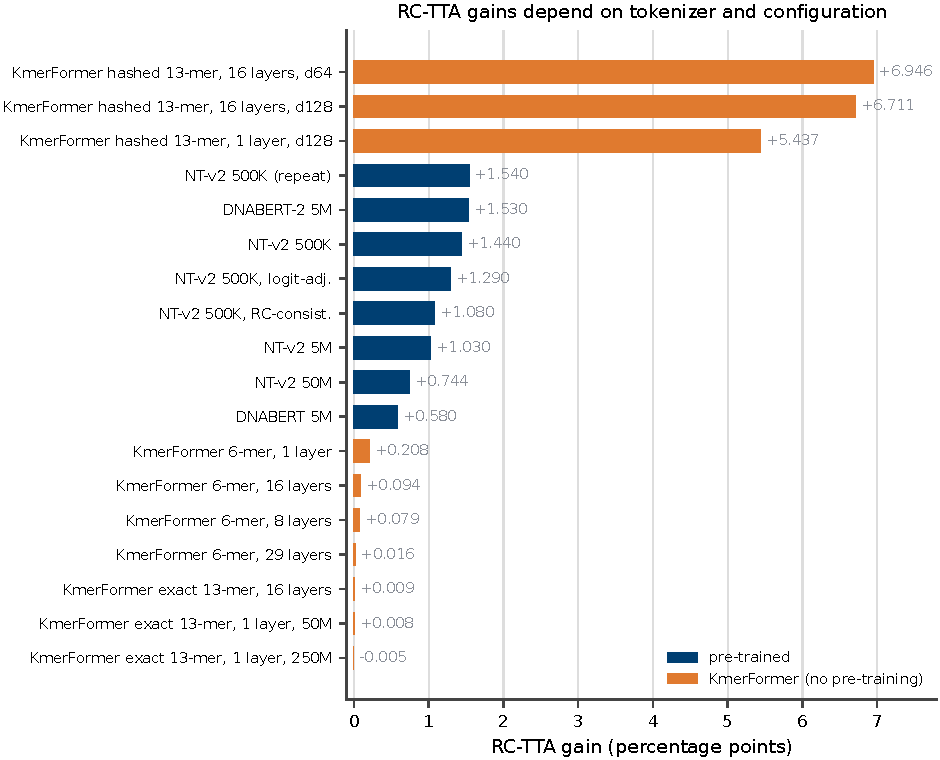
\includegraphics[width=\textwidth]{figures/rc_tta_benefit.pdf}
    \caption{RC TTA benefit across experiments. Top: forward-only vs.\ RC TTA accuracy (blue: NT-v2 backbone; green: DNABERT family; right of second dashed line: random init). Bottom: absolute gain in percentage points. NT-v2-based models gain $+0.77$--$+1.54$~pp consistently. DNABERT gains only $+0.58$~pp, likely because its overlapping 6-mer tokenization is inherently more RC-symmetric than NT-v2's non-overlapping 6-mer. DNABERT-2 (BPE tokenization) gains $+1.53$~pp, similar to early NT-v2 experiments. The randomly initialized Shallow-Genus gains only $+0.08$~pp, confirming that the benefit primarily corrects pre-training-induced strand biases.}
    \label{fig:rc-tta}
\end{figure}

\section{Computational Resource Analysis}
\label{sec:exp-resources}

\subsection{Observed Resource Usage}

\begin{table}[htbp]
    \centering
    \caption{Computational resource usage across experiments.}
    \label{tab:resources}
    \begin{tabular}{lrrr}
        \toprule
        \textbf{Metric} & \textbf{v3 (500K)} & \textbf{NT-Genus-5M} & \textbf{NT-Genus} \\
        \midrule
        GPU & V100 32GB & H100 80GB & H100 80GB \\
        Batch size & 32 & 32 & 256 \\
        VRAM peak (training) & 10.4 GB & $\sim$4.7 GB & $\sim$5 GB \\
        VRAM utilization & 32.5\% & 5.5\% & $<$7\% \\
        Train throughput & 1,128 r/s & $\sim$1,800 r/s & $\sim$1,825 r/s \\
        Inference throughput & --- & $\sim$5,100 r/s & $\sim$5,170 r/s \\
        Epoch time & $\sim$6.5 min & $\sim$6.8h & $\sim$6.9h \\
        Total training & 11.5h & $\sim$90h & $\sim$207h (30 ep.) \\
        SLURM jobs needed & 1 & 3 & 4+ \\
        \bottomrule
    \end{tabular}
\end{table}

\subsection{Bottleneck Analysis}

\begin{table}[htbp]
    \centering
    \caption{Resource bottleneck assessment on TWCC H100 nodes.}
    \label{tab:bottleneck}
    \begin{tabular}{lll}
        \toprule
        \textbf{Resource} & \textbf{Status} & \textbf{Assessment} \\
        \midrule
        GPU VRAM (80 GB) & $<$50\% utilized & No upgrade needed \\
        GPU compute (H100) & Adequate & No upgrade needed \\
        System RAM (128 GB) & $<$50\% utilized & No upgrade needed \\
        Storage & $<$10 GB per experiment & No upgrade needed \\
        \textbf{SLURM time (48h)} & \textbf{Primary bottleneck} & \textbf{Requires resume or longer limits} \\
        \bottomrule
    \end{tabular}
\end{table}

The hardware is substantially over-provisioned for this workload: the H100 80~GB GPU runs at $<$50\% VRAM utilization even with batch size 256, and system RAM usage is well within limits. The primary operational bottleneck is the 48-hour SLURM wall time limit, which necessitates multiple job submissions with checkpoint resumption for large-scale experiments.

\section{Comparison with MetaTransformer}
\label{sec:exp-comparison}

\begin{table}[htbp]
    \centering
    \caption{Comparison between our approach and MetaTransformer~\cite{Wichmann2023}.}
    \label{tab:metatransformer-comparison}
    \begin{tabular}{lcc}
        \toprule
        \textbf{Aspect} & \textbf{NT-Genus} & \textbf{MetaTransformer} \\
        \midrule
        Backbone & NT-v2 (498M) & Custom Transformer ($\sim$5M encoder$^\dagger$) \\
        Tokenization & 6-mer (pre-trained) & 12-mer (learned) \\
        Pre-training & Yes (850 genomes, MLM) & No (trained from scratch) \\
        Trainable params & 5.54M (LoRA) & $\sim$5M encoder$^\dagger$ (all) \\
        Training data & 50M balanced & HGR-UMGS full (2,505 sp., coverage 4) \\
        Genus accuracy & 67.07\% (RC TTA) & 98.3\% recall (val) \\
        Data source & HGR-UMGS + ART & HGR-UMGS + ART (same) \\
        \bottomrule
    \end{tabular}
    \begin{minipage}{\linewidth}
        \vspace{2pt}
        \footnotesize $^\dagger$Encoder parameters only; the embedding table is not counted here. For the overlapping 13-mer (stride~1) configuration, the embedding table alone is ${\sim}2.1$B parameters (see the parameter-accounting caveat below).
    \end{minipage}
\end{table}

Despite using a foundation model $100\times$ larger than MetaTransformer, our model (at 50M training reads) substantially underperforms MetaTransformer (trained on the full HGR-UMGS dataset). The key differences are:

\begin{enumerate}
    \item \textbf{Training data volume}: MetaTransformer uses the full HGR-UMGS dataset with coverage~4 vs. our 50M balanced reads. Inside the 6-mer framework each $10\times$ data increase yields $+3$--$8$~pp with diminishing returns, but the 250M run (Section~\ref{sec:exp-scaling}) shows that extra 6-mer data does not close this gap.
    
    \item \textbf{Training paradigm}: MetaTransformer trains all encoder parameters from scratch ($\sim$5M; the embedding table is additional---see parameter-accounting caveat below), while we fine-tune only 5.54M LoRA parameters of a 498M-parameter model.
    
    \item \textbf{Tokenization}: MetaTransformer uses 12-mer tokenization (capturing longer sequence patterns per token), while NT-v2 uses 6-mers.
\end{enumerate}

This comparison is confounded by three simultaneous differences: backbone depth (29 vs.\ 1 layer), pre-training (yes vs.\ no), and tokenization (6-mer vs.\ 12-mer overlapping). Sections~\ref{sec:exp-shallow} and~\ref{sec:exp-tokenization} separate these factors. Tokenization accounts for the larger share of the gap. The one-layer versus 29-layer comparison does \emph{not} isolate pre-training; the depth sweep in Section~\ref{sec:exp-shallow} does.

\paragraph{The ``$\sim$5M parameters'' figure counts only the encoder.}
The $\sim$5M parameter count attributed to MetaTransformer throughout this comparison refers to its \emph{transformer encoder} alone; it omits the token-embedding table, which for large-$k$ tokenization dominates the parameter budget. A learned $k$-mer embedding assigns a distinct vector to every $k$-mer observed in training, so the embedding matrix grows with the realized vocabulary. For the overlapping 13-mer (stride~1) configuration that attains 87.42\% at 50M and 98.7\% at 250M, the realized vocabulary reaches ${\sim}33.5$M distinct $k$-mers; at the embedding width $d_{\text{model}}{=}64$, the embedding matrix alone is ${\sim}33.5\text{M}\times 64 \approx 2.1$ billion parameters---roughly $4\times$ the size of the entire 498M-parameter NT-v2 backbone. The 13-mer model is therefore parameter-light only in \emph{compute} (a single shallow encoder block over short token sequences), while being parameter-\emph{heavy} in \emph{storage} (a multi-billion-entry lookup table). This is intrinsic to the approach: its discriminative power comes precisely from giving each long $k$-mer its own vector, which is also what inflates the table. A fair efficiency comparison must therefore weigh MetaTransformer's small compute footprint against this large embedding-memory cost, rather than citing the ${\sim}5$M encoder figure as the model's total size.

\section{Backbone Ablation: Depth, Then Pre-training}
\label{sec:exp-shallow}

A one-layer randomly initialized Transformer with the same 6-mer tokenizer and attention-pooling head as NT-v2 (Section~\ref{sec:method-shallow}) is the comparison originally used to ``isolate pre-training.'' It does not: encoder depth (29 vs.\ 1) and width ($d{=}1024$ vs.\ $d{=}128$) change at the same time as pre-training. We keep that comparison as a confounded baseline, then vary only depth.

\subsection{Confounded baseline: 29-layer NT-v2 vs.\ one-layer from scratch}

\begin{table}[htbp]
    \centering
    \caption{Confounded backbone comparison: NT-v2 (NT-Genus) vs.\ one-layer Transformer (Shallow-Genus). Tokenizer, head, and 50M reads are shared; depth, width, and pre-training are not.}
    \label{tab:shallow-design}
    \begin{tabular}{lcc}
        \toprule
        \textbf{Component} & \textbf{NT-Genus} & \textbf{Shallow-Genus} \\
        \midrule
        Tokenizer & 6-mer (NT-v2) & 6-mer (NT-v2) \\
        Encoder & 29-layer, $d{=}1024$ & 1-layer, $d{=}128$ \\
        Pre-training & MLM on 850 genomes & None \\
        Trainable params & 5.54M (LoRA) & $\sim$200K (all) \\
        Classification head & Attention pool (4 heads) & Attention pool (4 heads) \\
        Training data & 50M balanced & 50M balanced \\
        Batch size & 256 & 512 \\
        \bottomrule
    \end{tabular}
\end{table}

\begin{table}[htbp]
    \centering
    \caption{Confounded backbone results on the original 50M splits: pre-trained NT-v2 (NT-Genus) vs.\ one-layer Transformer (Shallow-Genus). The $-13.19$~pp RC-TTA gap is real; it is not an isolated pre-training effect.}
    \label{tab:v11-results}
    \begin{tabular}{lccr}
        \toprule
        \textbf{Metric} & \textbf{NT-Genus} & \textbf{Shallow-Genus} & \textbf{$\Delta$} \\
        \midrule
        Micro Accuracy (fwd) & 66.29\% & 53.80\% & $-12.49$~pp \\
        Micro Accuracy (RC TTA) & \textbf{67.07\%} & 53.88\% & $-13.19$~pp \\
        Balanced Accuracy & 39.91\% & 22.28\% & $-17.63$~pp \\
        F1 (macro) & 44.82\% & 25.78\% & $-19.04$~pp \\
        F1$=$0 classes & 0 & 3 & $+3$ \\
        RC TTA gain & $+0.78$~pp & $+0.08$~pp & --- \\
        Best epoch & 30 / 30 & 15 / 15 & --- \\
        Inference throughput & $\sim$5,170 r/s & $\sim$750,000 r/s & $\approx$145$\times$ \\
        VRAM (training) & $\sim$5 GB & $\sim$0.07 GB & --- \\
        \bottomrule
    \end{tabular}
\end{table}

NT-Genus outperforms Shallow-Genus by \textbf{13.19~pp} RC TTA (67.07\% vs.\ 53.88\%) on the original splits. Macro F1 drops more than micro accuracy ($-19.04$~pp vs.\ $-13.19$~pp). RC TTA is nearly ineffective for the randomly initialized model ($+0.08$~pp vs.\ $+0.78$~pp). Shallow-Genus is ${\sim}$145$\times$ faster at inference. None of these observations isolates pre-training from depth. Figure~\ref{fig:backbone-ablation} shows the same confounded pair.

\begin{figure}[htbp]
    \centering
    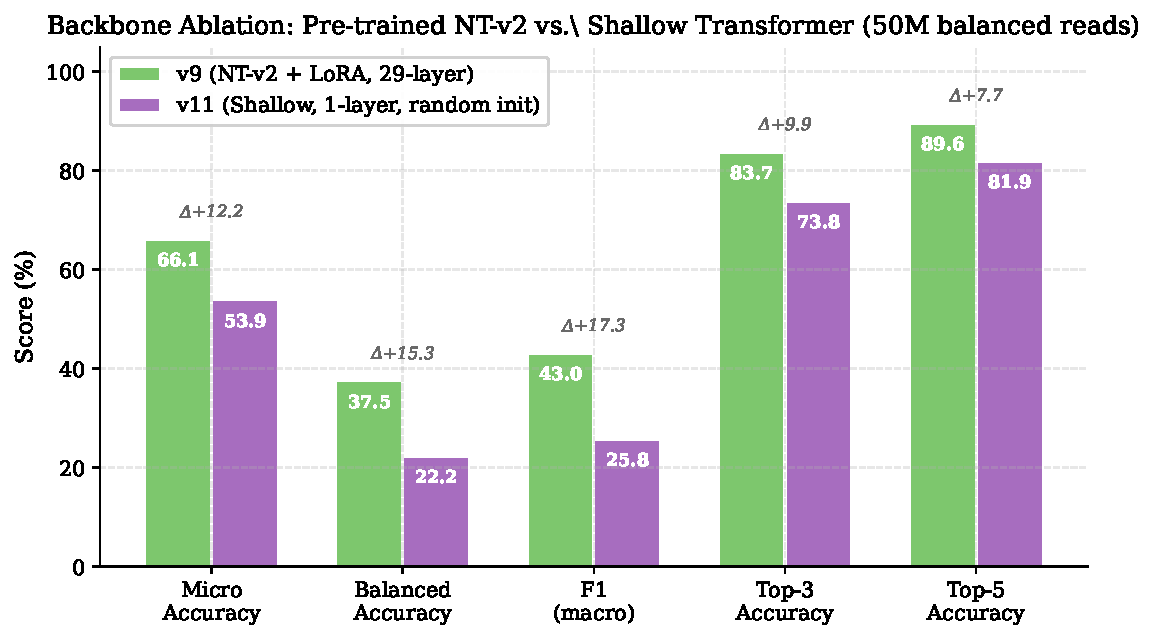
\includegraphics[width=0.90\textwidth]{figures/backbone_ablation.pdf}
    \caption{Confounded backbone comparison: pre-trained NT-v2 + LoRA (NT-Genus, green) vs.\ one-layer randomly initialized Transformer (Shallow-Genus, purple), both trained on 50M balanced reads. The gaps are real and include depth and width, not pre-training alone.}
    \label{fig:backbone-ablation}
\end{figure}

\subsection{Depth sweep at matched 6-mer tokenization}
\label{sec:exp-depth-sweep}

Table~\ref{tab:depth-sweep} holds the tokenizer (NT-v2 non-overlapping 6-mer), the 50M gut-read pool, the attention-pooling head, 15 training epochs, RC TTA, and the \texttt{clean\_common} 100K file fixed, and varies only encoder depth for the from-scratch models (Section~\ref{sec:method-shallow}). NT-v2 LoRA is the pre-trained reference on the same file.

\begin{table}[htbp]
    \centering
    \caption{Depth sweep, non-overlapping 6-mer, 50M gut reads, RC TTA on the same \texttt{clean\_common} 100K file. From-scratch models train 100\% of parameters. NT-v2 is LoRA-tuned (${\sim}$1\% of 500M).}
    \label{tab:depth-sweep}
    \small
    \begin{tabular}{lrrr}
        \toprule
        \textbf{Model} & \textbf{Params} & \textbf{Top-1} & \textbf{Balanced acc} \\
        \midrule
        1 layer, from scratch & 0.90M & 53.92\% & 0.220 \\
        8 layers, from scratch & 2.29M & 65.44\% & 0.388 \\
        16 layers, from scratch & 3.88M & \textbf{67.94\%} & \textbf{0.435} \\
        NT-v2, 29 layers, pre-trained + LoRA & 500M & 67.08\% & 0.398 \\
        \bottomrule
    \end{tabular}
\end{table}

Depth alone accounts for \textbf{+14.02~pp} (53.92\% $\to$ 67.94\%). That is larger than the $+13.19$~pp previously attributed to pre-training. The 16-layer from-scratch model \emph{exceeds} NT-v2 by $+0.86$~pp micro and $+3.7$~pp balanced accuracy with $129\times$ fewer parameters. A 3.88M-parameter model trained 100\% from scratch therefore matches the 6-mer ceiling of a 500M LoRA-tuned GFM; the ceiling is not an artefact of updating only ${\sim}$1\% of NT-v2. Neither from-scratch run had early-stopped at epoch 15, so the from-scratch numbers are lower bounds.

The one-layer re-run on \texttt{clean\_common} (53.92\%) agrees with the original Shallow-Genus 53.88\% on the internal split. NT-v2 on \texttt{clean\_common} (67.08\%) agrees with NT-Genus 67.07\%. The two pools match; the attribution does not.

For the 8-layer model, internal validation rose 0.634 $\to$ 0.654 from epoch 9 to 15 while \texttt{clean\_common} stayed at 65.44\%: the last six epochs memorised duplicated reads with no generalisation gain, consistent with the $6.07\times$ sequence-level redundancy in Section~\ref{sec:exp-setup}. Excluding the 0.17\% of \texttt{clean\_common} reads that share a \texttt{seq\_id} with training changes 65.44\% to 65.43\%.

\subsection{Data-efficiency crossover at matched depth}
\label{sec:exp-crossover}

The 50M result says pre-training does not raise the 6-mer ceiling. Table~\ref{tab:crossover-5m} asks whether it still helps when labels are scarce. A 16-layer from-scratch 6-mer model is trained on the same 5M gut reads used for NT-v2 v8 and scored on \texttt{clean\_common} with RC TTA.

\begin{table}[htbp]
    \centering
    \caption{Depth-matched 6-mer comparison at 5M gut reads (RC TTA). The 16-layer from-scratch model is scored on \texttt{clean\_common}. NT-v2 v8's 63.05\% is its recorded internal-validation figure (that checkpoint was not re-scored on \texttt{clean\_common}); models we could check agree across the two pools (8-layer 0.6539 / 65.44\%, 16-layer 0.6772 / 67.94\%, NT-v2 v9 0.6707 / 67.08\%), and the 16-layer 5M run itself scored 0.5411 on both.}
    \label{tab:crossover-5m}
    \small
    \begin{tabular}{lrr}
        \toprule
        \textbf{Model (5M, 6-mer)} & \textbf{Params} & \textbf{Top-1} \\
        \midrule
        8-layer from scratch & 2.29M & 53.62\% \\
        16-layer from scratch & 3.88M & 54.11\% \\
        NT-v2 v8, pre-trained + LoRA & 500M & \textbf{63.05\%} \\
        \bottomrule
    \end{tabular}
\end{table}

At 5M, going from 8 to 16 layers buys $+0.49$~pp; at 50M the same step is $+2.50$~pp. Depth needs data to pay off, so extra from-scratch depth would not close the low-data gap. Combined with Table~\ref{tab:depth-sweep}:

\begin{table}[htbp]
    \centering
    \caption{Depth-matched pre-training contribution (16-layer from-scratch vs.\ NT-v2, non-overlapping 6-mer). Pre-training buys data efficiency, not a higher 50M ceiling.}
    \label{tab:crossover-summary}
    \small
    \begin{tabular}{lccc}
        \toprule
        \textbf{Training reads} & \textbf{16-layer scratch} & \textbf{NT-v2} & \textbf{Net pre-training} \\
        \midrule
        5M  & 54.11\% & 63.05\% & \textbf{$+8.94$~pp} \\
        50M & \textbf{67.94\%} & 67.08\% & $-0.86$~pp \\
        \bottomrule
    \end{tabular}
\end{table}

Soil 50M comparisons of NT-v2 against a one-encoder-block MetaTransformer remain depth-confounded in the same way as Table~\ref{tab:v11-results}; they are not reported here as evidence for pre-training. Depth-matched soil controls were not completed.

\section{Tokenization Ablation: MetaTransformer at 50M Scale}
\label{sec:exp-tokenization}

The depth sweep (Section~\ref{sec:exp-shallow}) shows that, at matched 6-mer tokenization, pre-training does not raise the 50M ceiling. Tokenization is the remaining design difference relative to MetaTransformer. We first train the MetaTransformer architecture~\cite{Wichmann2023} on the same 50M balanced dataset under six tokenization configurations ($k \in \{6, 12, 13\}$, stride $\in \{1, k\}$), using the original MetaTransformer codebase on the Taiwania-2 cluster (V100 32~GB GPU). All configurations are evaluated on the same stratified 90/10 val split (5M reads). The 13-mer model uses \textit{embed\_dim}~$=$~64 to fit within V100 memory, consistent with the original MetaTransformer paper's 13-mer configuration~\cite{Wichmann2023}. A same-architecture 16-layer comparison in our codebase follows (Section~\ref{sec:exp-samearch-tok}).

\begin{table}[htbp]
    \centering
    \caption{Tokenization ablation (genus-level, 120 classes): NT-v2 + LoRA vs.\ MetaTransformer under six tokenization configurations. All MetaTransformer models are trained from scratch on 50M balanced reads. RC TTA is unavailable for MetaTransformer.}
    \label{tab:tokenization-ablation}
    \begin{tabular}{llccc}
        \toprule
        \textbf{Model} & \textbf{Tokenization} & \textbf{Tokens/read} & \textbf{Top-1 Acc} & \textbf{Macro F1} \\
        \midrule
        MetaTransformer & 13-mer, stride=1  & 138 & \textbf{87.42\%} & \textbf{0.7936} \\
        MetaTransformer & 12-mer, stride=1  & 139 & 78.83\% & 0.6531 \\
        NT-Genus & 6-mer, stride=6 & 25  & 67.07\%$^\dagger$ & --- \\
        NT-Genus & 6-mer, stride=6 & 25  & 66.29\% & 0.4384 \\
        MetaTransformer & 6-mer, stride=1   & 145 & 48.87\% & 0.1981 \\
        MetaTransformer & 6-mer, stride=6   & 25  & 47.00\% & 0.1682 \\
        MetaTransformer & 12-mer, stride=12 & 12  & 40.66\% & 0.0663 \\
        MetaTransformer & 13-mer, stride=13 & 11  & 27.30\% & 0.0182 \\
        \bottomrule
    \end{tabular}
    \begin{tablenotes}
        \small
        \item $\dagger$ RC TTA result (+0.78~pp over forward-only 66.29\%); MetaTransformer results are forward-only.
    \end{tablenotes}
\end{table}

\begin{table}[htbp]
    \centering
    \caption{Tokenization ablation (species-level, 1,535 classes): MetaTransformer under six tokenization configurations, trained on the same 50M balanced reads.}
    \label{tab:tokenization-ablation-species}
    \begin{tabular}{llccc}
        \toprule
        \textbf{Model} & \textbf{Tokenization} & \textbf{Tokens/read} & \textbf{Top-1 Acc} & \textbf{Macro F1} \\
        \midrule
        MetaTransformer & 13-mer, stride=1  & 138 & \textbf{49.62\%} & \textbf{0.4950} \\
        MetaTransformer & 12-mer, stride=1  & 139 & 16.79\% & 0.1439 \\
        MetaTransformer & 6-mer, stride=1   & 145 &  9.13\% & 0.0719 \\
        MetaTransformer & 6-mer, stride=6   & 25  &  6.44\% & 0.0470 \\
        MetaTransformer & 12-mer, stride=12 & 12  &  0.64\% & 0.0023 \\
        MetaTransformer & 13-mer, stride=13 & 11  &  0.51\% & 0.0026 \\
        \bottomrule
    \end{tabular}
\end{table}

Three independent effects can be read from Tables~\ref{tab:tokenization-ablation}--\ref{tab:tokenization-ablation-species}:

\paragraph{Effect of switching to the NT-v2 backbone (6-mer tokenization held; depth and codebase are not).}
NT-Genus (66.29\% forward) outperforms MetaTransformer with the same non-overlapping 6-mer tokenization (47.00\%) by \textbf{+19.29~pp}. This is an operational gap, not an isolated pre-training effect: MetaTransformer uses one encoder block, NT-v2 uses 29 layers, and the two codebases differ. Section~\ref{sec:exp-shallow} already showed that a 16-layer from-scratch 6-mer in our codebase reaches 67.94\%---above NT-v2---so MetaTransformer's 47.00\% 6-mer result understates the 6-mer ceiling. The number that isolates tokenization \emph{inside} MetaTransformer is the next paragraph, not this $+19.29$~pp.

\paragraph{Effect of tokenization (MetaTransformer architecture held constant).}
Tokenization design has a far larger effect than pre-training. Two sub-effects compound:
\begin{enumerate}
    \item \textbf{Stride (overlapping vs.\ non-overlapping)}: Across all $k$ values, overlapping stride$=$1 dominates non-overlapping stride$=k$. The gap widens dramatically with $k$: $+1.87$~pp for $k=6$, $+38.17$~pp for $k=12$, and $+60.12$~pp for $k=13$. Non-overlapping tokenization with large $k$ reduces each 150~bp read to as few as 11 tokens, discarding most sequence context.
    \item \textbf{k-mer length (overlapping only)}: Among stride$=$1 configurations, longer $k$ yields monotonically higher accuracy: 6-mer (48.87\%) $<$ 12-mer (78.83\%) $<$ 13-mer (87.42\%) at genus level, and 9.13\% $<$ 16.79\% $<$ 49.62\% at species level. Longer tokens are taxonomically more specific---hexamers are shared across distant taxa, while 12-mers and 13-mers increasingly identify individual lineages.
\end{enumerate}

\paragraph{Tokenization vs.\ NT-v2: MetaTransformer 13-mer.}
MetaTransformer with overlapping 13-mer tokenization, trained \emph{from scratch} on the 50M dataset (45M training reads), achieves \textbf{87.42\%} genus Top-1 accuracy---\textbf{+20.35~pp} above NT-Genus with RC TTA (67.07\%), with a transformer encoder ${\sim}100\times$ smaller and no pre-training (though its large-$k$ embedding table makes its \emph{total} parameter count far larger than NT-v2's; see the parameter-accounting caveat in Section~\ref{sec:exp-comparison}). Against the depth-matched 16-layer 6-mer (67.94\%), the best-vs-best gap is still ${\sim}$20~pp (87.42\% vs.\ 67.94\%), even though the 13-mer model uses one encoder block and the 6-mer model uses 16. At species level, MT 13-mer stride$=$1 reaches \textbf{49.62\%} (1,535 classes) on the 5M validation set and \textbf{49.74\%} on the independent 100K test set (Section~\ref{sec:spv4-hierarchical-prelim}), without any hierarchical routing. Task-specific tokenization is a more decisive factor than pre-trained prior knowledge for this task.

\paragraph{Decomposition from a common MetaTransformer 6-mer baseline.}
Because reverse-complement TTA is unavailable for MetaTransformer, Table~\ref{tab:pretraining-tokenization-decomp} changes one factor at a time from the from-scratch MetaTransformer non-overlapping 6-mer (47.00\% forward). The overlapping-12-mer and 13-mer rows hold the MetaTransformer architecture fixed and are therefore tokenization effects ($+31.83$~pp and $+40.42$~pp). The NT-v2 row does \emph{not} hold depth or codebase fixed; it is included only as the operational gap ($+19.29$~pp) that Section~\ref{sec:exp-shallow} already showed is not pre-training. Tokenization remains the largest single-factor change on this table.

\begin{table}[htbp]
    \centering
    \caption{Single-factor changes from a common from-scratch MetaTransformer 6-mer (non-overlapping) baseline at 50M reads (47.00\% forward genus Top-1). Overlapping 12-mer and 13-mer hold the MetaTransformer architecture fixed. The NT-v2 row additionally changes depth, width, pre-training, and codebase, and is not an isolated pre-training effect (Section~\ref{sec:exp-shallow}). All values are forward-only.}
    \label{tab:pretraining-tokenization-decomp}
    \small
    \begin{tabular}{lcc}
        \toprule
        \textbf{Single-factor change from MT 6-mer scratch (47.00\%)} & \textbf{Genus Top-1 (fwd)} & \textbf{$\Delta$} \\
        \midrule
        $+$ NT-v2 backbone (depth, pre-training, codebase also change)  & 66.29\% & $+19.29$~pp \\
        $+$ overlapping 12-mer tokenization (MT held)  & 78.83\% & $+31.83$~pp \\
        $+$ overlapping 13-mer tokenization (MT held)  & 87.42\% & $+40.42$~pp \\
        \bottomrule
    \end{tabular}
\end{table}

\paragraph{The bottleneck is representational: a train-fit ceiling.}
The decomposition above measures held-out accuracy, which conflates representational capacity with generalisation. A sharper test asks whether each model can fit its \emph{own training data}: a model that cannot separate the training set is limited by its input representation, not by capacity, data volume, optimisation, or overfitting. Table~\ref{tab:train-fit} reports training and validation accuracy at the largest (250M-read) scale. The NT-v2 6-mer models plateau at $63$--$66\%$ \emph{on the training set itself}, essentially equal to their validation accuracy (train--val gap ${\le}1$~pp)---they are not overfitting, they simply cannot fit. By contrast, MetaTransformer with overlapping 13-mer tokenisation fits the same task to $98.9\%$ training accuracy ($97.5\%$ validation).

The implication is decisive: with non-overlapping 6-mer tokenisation, reads from different genera are mapped to token sequences too similar to be separated, so no amount of additional capacity, data, or training can raise accuracy---the ceiling is imposed before learning begins, by the tokenizer. Overlapping 13-mers preserve enough sequence detail that the \emph{same model family} fits the data almost perfectly. This train-fit ceiling is the strongest single piece of evidence that tokenization, rather than backbone capacity or data volume, is the operative bottleneck for 6-mer GFMs on this task.

\begin{table}[htbp]
    \centering
    \caption{Train-fit ceiling at 250M reads: the 6-mer models cannot fit the training set beyond ${\sim}66\%$, whereas an overlapping 13-mer model fits it to ${\sim}99\%$. Training and validation accuracy are essentially equal for the 6-mer models, ruling out overfitting and isolating the input representation as the bottleneck. NT-v2 figures are forward micro-accuracy; the MetaTransformer training figure is micro-precision.}
    \label{tab:train-fit}
    \small
    \begin{tabular}{lccc}
        \toprule
        \textbf{Model (250M reads)} & \textbf{Train acc} & \textbf{Val acc} & \textbf{Train--val gap} \\
        \midrule
        NT-v2 6-mer, from scratch        & 63.2\% & 64.1\% & $-0.9$~pp \\
        NT-v2 6-mer, warm-start          & 65.8\% & 66.6\% & $-0.8$~pp \\
        MetaTransformer 13-mer (overlap) & \textbf{98.9\%} & \textbf{97.5\%} & $+1.4$~pp \\
        \bottomrule
    \end{tabular}
\end{table}

\paragraph{Convergence and capacity ceiling (12-mer).}
To determine whether 78.83\% is the true ceiling for the 12-mer model, training was extended into a second epoch. Train loss dropped sharply from 0.764 to 0.119, while validation loss \emph{worsened} from 1.203 to 2.288---immediate overfitting. The 50M-read dataset saturates the 5M-parameter single-encoder MetaTransformer within one epoch.

\paragraph{Overlapping tokenization within pre-trained GFMs (5M scale).}
The MetaTransformer ablation above is conducted entirely from scratch at 50M scale.
To isolate the effect of overlapping tokenization \emph{within the pre-trained GFM family}, we additionally fine-tune two other pre-trained DNA language models on the same 5M balanced dataset using identical training settings (LoRA $r=16$, attention-pooling head):
\begin{itemize}
    \item \textbf{DNABERT}~\cite{Ji2021}: BERT-base (86M params) pre-trained on the human reference genome with overlapping 6-mer tokenization (stride$=$1, 145 tokens per 150~bp read).
    \item \textbf{DNABERT-2}~\cite{Zhou2024dnabert2}: BERT-base (117M params) pre-trained on a multi-species genome collection using learned BPE tokenization ($\sim$34 tokens per read).
\end{itemize}

\begin{table}[htbp]
    \centering
    \caption{Pre-trained GFM backbone comparison at 5M balanced reads (genus-level, 120 classes).
    All models use LoRA $r=16$ fine-tuning and the same attention-pooling head.
    RC TTA is applied to all models.}
    \label{tab:backbone-tokenization-5M}
    \small
    \setlength{\tabcolsep}{4pt}
    \begin{tabular}{llcccc}
        \toprule
        \textbf{Model} & \textbf{Tokenization} & \textbf{Tokens/read} & \textbf{Params} & \textbf{RC TTA Acc} & \textbf{Macro F1} \\
        \midrule
        NT-Genus-5M  & 6-mer ($s{=}6$, non-overlap) & 25       & 499M & \textbf{63.05\%} & \textbf{0.449} \\
        DNABERT + LoRA     & 6-mer ($s{=}1$, overlap)     & 145      & 86M  & 61.78\%          & 0.384 \\
        DNABERT-2 + LoRA   & BPE                          & $\sim$34 & 117M & 58.88\%          & 0.323 \\
        \bottomrule
    \end{tabular}
\end{table}

Three observations follow from Table~\ref{tab:backbone-tokenization-5M}.

First, NT-Genus-5M with \emph{non-overlapping} 6-mer tokenization outperforms DNABERT with \emph{overlapping} 6-mer tokenization by $+1.27$~pp.
At 5M training reads, the pre-training advantage from NT-v2's larger backbone (499M vs.\ 86M parameters) and more diverse pre-training corpus (850 microbial genomes vs.\ human genome only) outweighs the tokenization benefit of overlapping stride.
This contrasts with the MetaTransformer results: when starting from scratch on the same data, overlapping tokenization provides a large benefit ($+1.87$~pp at $k=6$, $+60.12$~pp at $k=13$); but when starting from a strong pre-trained representation, the non-overlapping NT-v2 backbone already captures sufficient local context through its positional encodings.

Second, DNABERT with overlapping 6-mer tokenization (pre-trained, 86M, 5M data, 61.78\%) outperforms MetaTransformer with the same overlapping 6-mer tokenization (from scratch, one encoder block, 50M data, 48.87\%), despite ten times less training data.
This is an operational data-efficiency comparison at matched $k$; it is not depth-matched, and it should not be read as the isolated pre-training effect already measured in Section~\ref{sec:exp-crossover}.

Third, DNABERT-2's BPE tokenization (58.88\%) performs worse than either 6-mer model despite having a similar parameter count to DNABERT.
BPE segments DNA by frequency-based byte pairs rather than fixed-length k-mers, which may fragment taxonomically informative motifs; the learned vocabulary may not align well with the k-mer statistics that distinguish metagenomic reads.

\paragraph{Methodological note on training equivalence.}
The three models use the same learning rate ($5\times10^{-4}$ head/LoRA, $3\times10^{-5}$ backbone), warmup ratio (5\%), cosine decay schedule, and epoch count (30), but differ in batch size (NT-v2: 32, DNABERT: 128, DNABERT-2: 256) due to GPU memory constraints imposed by sequence length differences (25, 145, and $\sim$34 tokens per read respectively).
Consequently, the total number of gradient updates differs: approximately 453K for NT-v2, 117K for DNABERT, and 59K for DNABERT-2.
All three learning curves were still improving at epoch 30 (gain $<0.1$~pp per epoch), with the cosine schedule decaying the learning rate to near zero by the final epoch.
The comparison is therefore epoch-based---each model has seen the training data 30 times---rather than step-based or compute-matched.
This is standard practice in fine-tuning comparisons, and the observed ranking (NT-v2 $>$ DNABERT $>$ DNABERT-2) is unlikely to be reversed by additional training: DNABERT, despite receiving 3.9$\times$ fewer gradient updates than NT-v2, lags by only $1.27$~pp, while DNABERT-2's gap of $4.17$~pp is consistent across all training stages and attributable primarily to its BPE tokenization.

\paragraph{Sample-level evaluation of the three GFM backbones (5M scale).}
Read-level accuracy alone does not capture how a backbone choice propagates to the sample-level abundance and detection metrics that matter in practice.
We therefore apply the sample-level evaluation protocol (5M validation pool, 50K reads per sample, 100 partition samples; Section~\ref{sec:exp-sample}) to the RC-TTA predictions of all three pre-trained backbones at 5M scale.
Table~\ref{tab:backbone-sample-5M} reports the results.

\begin{table}[htbp]
    \centering
    \caption{Sample-level genus evaluation of the three pre-trained GFM backbones at 5M balanced reads (RC TTA predictions, 5M validation pool, 50K reads/sample).}
    \label{tab:backbone-sample-5M}
    \small
    \setlength{\tabcolsep}{5pt}
    \begin{tabular}{lccccc}
        \toprule
        \textbf{Model} & \textbf{Read Acc} & \textbf{Pearson $r$} & \textbf{Bray-Curtis} & \textbf{ROC AUC} & \textbf{Sens @ 95\% Spec} \\
        \midrule
        NT-Genus-5M       & \textbf{63.05\%} & \textbf{0.9928} & \textbf{0.112} & 0.666 & \textbf{14.5\%} \\
        DNABERT + LoRA    & 61.78\%          & 0.9906          & 0.113          & \textbf{0.672} & 14.2\% \\
        DNABERT-2 + LoRA  & 58.88\%          & 0.9915          & 0.141          & 0.640 & 11.6\% \\
        \bottomrule
    \end{tabular}
\end{table}

Two patterns emerge.
First, abundance estimation (Pearson $r$) saturates at $\sim$0.99 for all three backbones, consistent with the genus-level finding that relative-abundance correlation is forgiving at low task granularity (Section~\ref{sec:sample-mt-comparison})---the read-accuracy ranking (NT-Genus $>$ DNABERT $>$ DNABERT-2) does not separate the backbones on Pearson $r$.
Second, the discriminating metrics are Bray-Curtis dissimilarity and binary detection: DNABERT-2 is clearly worst on both (Bray-Curtis 0.141 vs.\ 0.112--0.113; ROC AUC 0.640 vs.\ 0.666--0.672; sensitivity at 95\% specificity 11.6\% vs.\ 14.2--14.5\%), mirroring its lower read accuracy and reinforcing that BPE tokenisation is the weakest of the three for this task.
NT-Genus and DNABERT are nearly indistinguishable at the sample level, with NT-Genus marginally ahead on Bray-Curtis and sensitivity and DNABERT marginally ahead on ROC AUC.

\paragraph{Same-architecture tokenizer comparison (16 layers).}
\label{sec:exp-samearch-tok}
The MetaTransformer $k$/stride grid holds one codebase fixed. Table~\ref{tab:samearch-tok} holds \emph{our} 16-layer encoder, the 50M gut-read pool, and \texttt{clean\_common} RC TTA fixed, and varies only the tokenizer (Section~\ref{sec:method-samearch-tok}). All three Taiwania-2 arms (Jobs~A/B/C) trained the full 15 epochs.

\begin{table}[htbp]
    \centering
    \caption{Same-architecture tokenizer comparison on 50M gut reads, scored on \texttt{clean\_common} 100K with RC TTA. The 16-layer non-overlapping 6-mer and 29-layer 6-mer rows are local runs; Jobs~A/B/C were trained on Taiwania-2. MetaTransformer 13-mer is the one-block published-protocol number from Table~\ref{tab:tokenization-ablation}, not a 16-layer run.}
    \label{tab:samearch-tok}
    \small
    \setlength{\tabcolsep}{3.5pt}
    \begin{tabular}{llrccc}
        \toprule
        \textbf{Model} & \textbf{Tokenizer} & \textbf{Params} & \textbf{Tok/read} & \textbf{Top-1} & \textbf{Bal.\ acc} \\
        \midrule
        16L from scratch & overlap 6-mer (Job~B) & 3.88M & 146 & 62.75\% & 0.353 \\
        16L from scratch & non-overlap 6-mer & 3.88M & 25 & 67.94\% & 0.435 \\
        29L from scratch & non-overlap 6-mer & 6.45M & 25 & 69.52\% & 0.462 \\
        NT-v2 + LoRA & non-overlap 6-mer & 500M & 25 & 67.08\% & 0.398 \\
        16L from scratch & hashed 13-mer, 2~GiB (Job~C) & 540M & 139 & 83.83\% & 0.669 \\
        16L from scratch & exact 13-mer, 8.6~GiB (Job~A) & 2.15B & 139 & 85.63\% & 0.732 \\
        MetaTransformer (1 block) & exact 13-mer & --- & 139 & 87.42\% & --- \\
        \bottomrule
    \end{tabular}
\end{table}

Four results follow.

(i)~\textbf{Long $k$ works at matched depth.} Hashed 13-mer reaches \textbf{83.83\%}---$+15.89$~pp over the 16-layer non-overlapping 6-mer and $+16.75$~pp over NT-v2---with a 2~GiB embedding rather than the 48~GiB a dense $4^{13}$ table would need. Hashing costs \textbf{1.80~pp} versus the exact table (85.63\%). Macro F1 rises faster than Top-1: overlapping 6-mer Job~B has macro F1 0.385, hashed 13-mer 0.732 ($1.90\times$), exact 13-mer 0.747. The 6-mer long tail, not just Top-1, is the tokenizer.

(ii)~\textbf{Depth compensates for a weak tokenizer.} With a 6-mer tokenizer, $1\to 29$ layers is worth $+15.60$~pp (53.92\% $\to$ 69.52\%). With a 13-mer tokenizer, MetaTransformer reaches 87.42\% with one encoder block while our 16-layer exact 13-mer reaches 85.63\%. Depth and pre-training were substituting for a representation that discards the signal. A one-layer hashed 13-mer in our codebase was not run; MetaTransformer's 87.42\% protocol is the 50M matched run in Table~\ref{tab:tokenization-ablation}, not an independent re-implementation.

(iii)~\textbf{Overlapping 6-mer is harmful.} Overlapping 6-mer (146 tokens) scores \textbf{62.75\%}, $-5.19$~pp against non-overlapping 6-mer (25 tokens) at far higher compute. $k$ length, not overlap at $k=6$, is what matters here. This does not contradict the MetaTransformer result that overlap is essential at $k=12$/$13$: those non-overlapping settings collapse to 11--12 tokens per read.

(iv)~\textbf{Caveats.} Job~A differs from B/C in exact vs.\ hashed vocabulary, $d_{\text{model}}$ 64 vs.\ 128 (memory-forced), and a canonical (RC-invariant) vocabulary. The width confound favours C, so the exact-vocabulary advantage is not a width artefact. Job~A ran fp16; B and C ran bf16. Only \texttt{evaluate.py --rc\_tta} on \texttt{clean\_common} 100K is comparable across arms. Canonical-vocabulary analysis predicted RC-TTA behaviour before the numbers existed: Job~A $+0.01$ (TTA is a no-op), Job~C $+6.71$ (non-canonical hashing), Job~B $-0.03$ (\texttt{rc\_augment} already taught invariance).

\paragraph{Implication for NT-v2.}
NT-v2 is constrained to 6-mer tokenization by its pre-training design. Switching to overlapping 13-mer tokenization on the same 50M reads yields $+15.89$~pp (hashed, 16-layer) to $+20.35$~pp (MetaTransformer) without using NT-v2 pre-training. A genomic foundation model pre-trained with overlapping long-$k$ tokenization on microbial genomes would combine that tokenizer with pre-training as a data-efficiency mechanism (Section~\ref{sec:exp-crossover}). General-purpose GFMs of the NT-v2/DNABERT family do not currently provide that combination; METAGENE-1 and GenomeOcean use BPE and were not tested (Chapter~\ref{ch:conclusion}).

\section{Species-Level Classification at Scale}
\label{sec:exp-species-scaled}

Genus accuracy saturates near 67\% under 6-mer tokenization (Section~\ref{sec:exp-scaling}). Species classification (1{,}535 classes) is the stricter test of whether the same representation can resolve intra-genus variation. A 500K pilot reached only 8.32\% direct Top-1 and 20.88\% under oracle-genus masking---far above chance (0.065\%) but too data-starved to interpret---so the remainder of this section uses the 50M scale.

\subsection{NT-Species at 50M}
\label{sec:spv4-final}

The species model is initialized from the NT-Genus backbone (\texttt{--init\_from}), transferring LoRA weights and replacing the 120-way head with a 1{,}535-way head. Training converged at epoch~30 (Figure~\ref{fig:learning-curves}, right panel) to \textbf{17.55\%} forward Top-1 on the 5M held-out set, with Top-3/5/10 of 31.26\%/38.19\%/47.65\%, balanced accuracy 17.56\%, macro F1 0.157, and 191/1{,}535 species at F1~$=$~0 (12.4\%). The same learning-rate restart that affected NT-Genus appeared at epoch~7 ($-0.79$~pp) and was corrected from epoch~13. Full-scale RC~TTA and routing on all 5M reads exceeded the 200~GB memory ceiling of the evaluation script (it materialises $5\text{M}\times 1{,}535$ logit arrays per mode); hierarchical comparisons therefore use the independent 100K set below. The genus-level RC~TTA gain is already measured at $+0.78$~pp (Section~\ref{sec:exp-v9}).

\subsection{Independent Test Set and Data-Leakage Audit}
\label{sec:spv4-data-leakage}

Hierarchical modes restrict the candidate set, so even modest train--test overlap can inflate oracle and per-genus scores. The 100K subset first used for these modes had been sampled from the training FASTA \emph{before} the train/validation split and shared $>$99\% of reads with the 45M training pool. We replaced it with 100K reads from MetaTransformer's \texttt{val\_reads.fa}---the same ART protocol and 2{,}505 HGR-UMGS genomes, 0\% overlap with our training stream. Re-scoring NT-Genus gave 66.6\% on the overlapping 100K versus 66.1\% on the independent 100K ($0.5$~pp); the NT-Species flat baseline moved by less than $0.4$~pp. That is evidence against read-level memorisation, but all hierarchical numbers below use the independent set. Genus results in Section~\ref{sec:exp-v9} use the standard 5M validation split and are unaffected.

\subsection{Hierarchical Evaluation}
\label{sec:spv4-hierarchical-prelim}

Table~\ref{tab:hierarchical-prelim} reports every routing mode on the independent 100K set. NT-Genus is 66.1\% on this set. The MetaTransformer hierarchical rows use one genus model plus per-genus logit masking, not a per-genus ensemble.

\begin{table}[htbp]
    \centering
    \caption{Species Top-1 on the independent 100K-read test set (1{,}535 classes). Per-genus (50M) is 81 dedicated NT-v2 heads with a frozen backbone. MT hierarchical uses a single genus router and species-logit masking.}
    \label{tab:hierarchical-prelim}
    \small
    \begin{tabular}{llcc}
        \toprule
        \textbf{Model} & \textbf{Mode} & \textbf{Top-1} & \textbf{F1 (macro)} \\
        \midrule
        NT-Species (ep30) & Flat & 15.9\% & 0.135 \\
        & Top-5 / soft genus routing & 15.9\% / 15.8\% & 0.136 / 0.135 \\
        & Oracle (true genus) & 27.4\% & 0.252 \\
        \midrule
        Per-genus (50M) & Predicted genus (NT-Genus) & 15.6\% & 0.152 \\
        & Oracle genus & 29.5\% & 0.283 \\
        \midrule
        MT 13-mer ($s{=}1$) & Flat / hierarchical (87.5\% genus) & 49.74\% / \textbf{50.86\%} & --- \\
        MT 6-mer ($s{=}1$) & Flat / hierarchical (48.9\% genus) & 9.22\% / 6.41\% & --- \\
        \bottomrule
    \end{tabular}
\end{table}

Four conclusions follow, and they are all that the extra routing experiments add.

\textbf{Per-genus specialisation is real under a perfect router.} Oracle-genus routing lifts the 81 per-genus 50M classifiers to 29.5\% Top-1 (macro F1 0.283), above the flat NT-Species oracle (27.4\%, F1 0.252). The specialists use a \emph{frozen} backbone, so the gain is from decomposing the 1{,}535-way problem, not from extra fine-tuning.

\textbf{Predicted routing does not realise that gain.} With NT-Genus (66.1\%), the per-genus pipeline is 15.6\%, $0.3$~pp \emph{below} the flat 15.9\% baseline. A wrong genus sends the read to a candidate set that cannot contain the true species. Flat top-5 / soft routing moves Top-1 by at most $0.1$~pp. The binding constraint is genus accuracy, not the species head.

\textbf{Tokenization sets a higher ceiling than routing can recover.} MT overlapping 13-mer, with no hierarchical routing, reaches \textbf{49.74\%} on the same set---$+20.2$~pp above the best NT-v2 number under any routing mode (29.5\%). The 6-mer intra-genus ceiling sits in the high-20s; long-$k$ tokenization more than doubles it.

\textbf{Masking helps only when the router is already strong.} MT 13-mer genus accuracy is 87.5\%, and masking adds $+1.12$~pp (49.74\%~$\to$~50.86\%). MT 6-mer genus accuracy is 48.9\%, and the same masking \emph{costs} $2.81$~pp (9.22\%~$\to$~6.41\%). NT-v2 sits in between: oracle $+11.5$~pp on the flat model, predicted routing $-0.3$~pp on the specialists. Hierarchical masking is beneficial if and only if it removes more wrong candidates than it accidentally excludes.

\label{sec:spv4-per-genus}
The 81 multi-species heads were trained on genus-scoped 50M subsets ($\sim$32{,}600 reads per species) with the backbone frozen; 39 singleton genera are assigned deterministically. Mean per-genus validation accuracy is 48.3\% (median 44.2\%), but four large genera dominate the error: \textit{Collinsella} (349 species, 1.3\%), \textit{Clostridium} (191, 19.9\%), \textit{Prevotella} (91, 26.6\%), and \textit{Bacteroides} (79, 15.9\%). Genera with $\leq$5 species average $>$80\%; those with $>$50 species average $<$20\%.

\subsection{Subgenus Routing: A Negative Result}
\label{sec:subgenus-routing}

We tested whether a $K$-means partition of NT-v2 embeddings ($\sim$25--30 species per subgroup, including \textit{Blautia}) could shrink those large genera. For \textit{Collinsella} the silhouette coefficient is $0.03$; a UMAP projection is an undifferentiated blob. Hard and soft subgenus routing both \emph{lower} species Top-1 relative to the per-genus baseline they were compared against (predicted 14.7\%~$\to$~13.2\%/13.6\%; oracle 27.8\%~$\to$~25.6\%/26.1\%). The finalised per-genus numbers in Table~\ref{tab:hierarchical-prelim} are 15.6\%/29.5\%; the negative conclusion is unchanged. Adding a routing tier without a representation that separates species is counterproductive. The bottleneck is 6-mer within-genus resolution, not hierarchy depth.

\section{Sample-Level Application Evaluation}
\label{sec:exp-sample}

Per-read accuracy is not the quantity most metagenomic studies report. This section asks whether the 67.07\% NT-Genus model, and the species models above, produce usable relative abundances and presence/absence calls. Metrics follow CAMI and Bracken practice~\cite{Sczyrba2017,Meyer2022cami2,Lu2017,McIntyre2017}: Pearson $r$ and Spearman $\rho$ for abundance, Bray--Curtis dissimilarity for magnitude-aware error, and ROC AUC for detection. All genus numbers reuse the NT-Genus RC~TTA predictions of Section~\ref{sec:exp-v9}; no extra GPU inference is required.

Two synthetic constructions are taken from the 5M validation pool (120 genera). \textbf{Random-partition} samples (100 $\times$ 50{,}000 reads) keep every genus present; because training is species-balanced, the expected abundance of genus $g$ is $n_g/1{,}535$. \textbf{Sparse-community} samples (200 $\times$ 50{,}000 reads) include exactly 60 of 120 genera, supplying true negatives for detection.

\subsection{Genus Abundance and Detection}
\label{sec:sample-abundance}
\label{sec:sample-detection}

On the 100 random-partition samples, NT-Genus yields Pearson $r = 0.9932$ (std $0.0004$), Spearman $\rho = 0.9312$ (std $0.0080$), and Bray--Curtis $0.0937$ (std $0.0017$). A 33\% per-read error rate still aggregates, because misclassifications spread across genera and largely cancel. High-abundance genera are slightly overestimated (classifier bias toward genera with more member species), not because of genome-length artefacts in the ART schedule (Section~\ref{sec:method-data}).

That $r = 0.993$ is \emph{not} a test of variable communities. Every partition sample shares the same expected abundance profile; the correlation measures stability under binomial sampling noise. Sparse-community detection is the stricter probe. With a $\geq$1-read call, sensitivity is 93.9\% at 0.01--0.1\% true abundance, 97.6\% at 0.1--1\%, and 100\% at $\geq$1\%. ROC AUC with predicted abundance as the score is $0.705$; sensitivity is 17.2\%/30.9\%/46.2\% at 95\%/90\%/80\% specificity. The modest AUC is a noise floor: at 33\% error, an absent genus in a 50{,}000-read sample is expected to receive $\sim 50{,}000 \times 0.33 / 120 \approx 138$ spurious reads ($\sim$0.28\%). A 95\%-specificity threshold must sit at 1.49\% predicted abundance and therefore also suppresses genuinely rare taxa. Abundance estimation is forgiving at 120 classes; calibrated presence/absence is not.

\subsection{Matched Protocol across Models}
\label{sec:sample-mt-comparison}

Table~\ref{tab:sample-model-comparison} repeats the same sample protocol for NT-Genus and two MetaTransformer checkpoints trained on the same 50M reads.

\begin{table}[htbp]
    \centering
    \caption{Genus sample-level evaluation under one protocol (100 partition samples, 200 sparse samples, 50K reads). Read accuracies are 67.07\% (NT-Genus, RC~TTA), 48.82\% (MT 6-mer $s{=}1$), and 87.42\% (MT 13-mer $s{=}1$).}
    \label{tab:sample-model-comparison}
    \begin{tabular}{lccc}
        \toprule
        \textbf{Metric} & \textbf{NT-Genus} & \textbf{MT 6-mer} & \textbf{MT 13-mer} \\
        \midrule
        Pearson $r$ (abundance)   & 0.993 & 0.984 & \textbf{0.999} \\
        Bray--Curtis              & 0.094 & 0.167 & \textbf{0.028} \\
        Sensitivity $\geq$1\%     & 100\% & 99.9\% & \textbf{100\%} \\
        Sensitivity 0.1--1\%      & 97.6\% & 86.8\% & \textbf{100\%} \\
        ROC AUC                   & 0.705 & 0.569 & \textbf{0.900} \\
        Sensitivity @ 95\% spec   & 17.2\% & 9.4\% & \textbf{47.7\%} \\
        \bottomrule
    \end{tabular}
\end{table}

Relative abundance at genus rank barely separates the methods ($r = 0.984$--$0.999$). Detection does: MT 13-mer AUC $0.900$ versus $0.705$/$0.569$ for the two 6-mer models, matching the noise-floor arithmetic (expected spurious reads fall from $\sim$138 at 67\% accuracy to $\sim$54 at 87\%). NT-Genus beats the from-scratch 6-mer MetaTransformer on every sample metric; the two models also differ in depth, width, and codebase, so this is an operational comparison at matched $k$, not an isolated pre-training effect (Section~\ref{sec:exp-shallow}).

\subsection{Species-Level Samples and Kraken2}
\label{sec:sample-species}

The independent 100K set has only $\sim$65 reads per species, so samples are smaller (1{,}000 reads; 100 partitions; 50 genera present in sparse samples). Table~\ref{tab:sample-species-comparison} keeps the rows that change the conclusion.

\begin{table}[htbp]
    \centering
    \small
    \caption{Species-level sample evaluation on the independent 100K set (1{,}535 classes, 1K reads/sample). Kraken\,2 uses a custom $k{=}35$ database from the same 2{,}505 UMGS+HGR genomes; unclassified reads (30\%) count in the denominator but add zero predicted abundance. The MT 13-mer hierarchical species checkpoint did not converge (val\_loss $= 9.29$ at batch 10{,}000) and is omitted here; its read-level numbers in Table~\ref{tab:hierarchical-prelim} remain valid.}
    \label{tab:sample-species-comparison}
    \begin{tabular}{lcccc}
        \toprule
        \textbf{Model} & \textbf{Read Acc} & \textbf{Pearson $r$} & \textbf{Bray--Curtis} & \textbf{ROC AUC} \\
        \midrule
        NT-Species flat & 17.8\% & 0.135 & 0.589 & 0.794 \\
        NT-Species hierarchical & 15.8\% & 0.106 & 0.608 & 0.796 \\
        Per-genus (predicted / oracle) & 15.6\% / 29.5\% & 0.083 / 0.159 & 0.625 / 0.541 & 0.789 / 0.842 \\
        MT 6-mer flat / hierarchical & 9.0\% / 6.4\% & 0.066 / 0.041 & 0.652 / 0.682 & 0.692 / 0.639 \\
        MT 13-mer flat & 53.7\% & \textbf{0.503} & \textbf{0.353} & 0.973 \\
        Kraken\,2 (in-DB) & \textbf{66.2\%} & \textbf{0.727} & \textbf{0.218} & 0.925 \\
        \bottomrule
    \end{tabular}
\end{table}

At 1{,}535 classes a 1{,}000-read sample gives $\sim$0.65 true reads per species. NT-Species at 17.8\% therefore has a noise floor ($\sim$0.54 spurious reads per species) comparable to the signal, and Pearson $r$ stalls at $0.135$. MT 13-mer at 53.7\% reaches $r = 0.503$. Species-level abundance becomes useful only around 40--50\% per-read accuracy---a threshold 6-mer models in this thesis never cross and overlapping 13-mer does. Predicted hierarchical masking again hurts when the router is weak (NT-Genus 66.1\%: $r$ $0.135\to 0.106$; MT 6-mer 48.9\%: $0.066\to 0.041$). Oracle per-genus routing is the NT-v2 ceiling ($29.5$\%, $r = 0.159$) and remains $24.2$~pp of read accuracy behind MT 13-mer flat.

Kraken\,2 on the same references reaches 66.2\% species Top-1 and $r = 0.727$, committing to 70\% of reads (94.6\% species / 99.3\% genus among those). The remaining 30\% abstain. Restricting to the 85{,}819 reads whose species are in the Kraken\,2 FASTA collection (219 of 1{,}535 species had no local assembly) raises Kraken\,2 to 77.18\% species Top-1 versus 52.64\% for MT 13-mer flat. At \emph{genus} rank the comparison flips for uncorrected Kraken\,2 counts (NT-Genus $r = 0.992$, MT 13-mer $r = 0.9993$, raw Kraken\,2 $r = 0.823$ on that restricted pool), but Bracken~\cite{Lu2017} restores Kraken\,2$+$Bracken to $r = 0.997$. Neural models therefore have \emph{no} sample-level abundance advantage against a standard Kraken\,2$+$Bracken pipeline on these simulated communities. What remains is (i)~read-level accuracy under a suitable tokenizer and (ii)~the fact that a neural classifier trains from labelled reads and does not need a per-species reference FASTA---Kraken\,2 accuracy on the 14{,}181 uncovered GCF reads is 0\% by construction, whereas those species are in-distribution for every neural model here.

The practical summary is short. Genus relative abundance on synthetic, near-balanced partitions cannot choose a method. Species abundance requires a tokenizer that already clears $\sim$50\% read accuracy. Hierarchical experts and subgenus routing do not lift a 6-mer GFM above that line. Kraken\,2$+$Bracken matches neural genus abundances on in-database simulated reads; learning-based methods earn their keep only where assemblies are missing or the tokenizer is long-$k$.

\section{Summary of Findings}

The experimental results lead to several key conclusions:

\begin{enumerate}
    \item \textbf{Inside a fixed 6-mer tokenizer, data volume dominates tricks}: A $10\times$ data increase yields $+7.76$~pp, while training-technique optimizations yield at most $\pm0.5$~pp. Beyond 50M the 6-mer model saturates ($+0.22$~pp at 250M); an overlapping 13-mer does not.

    \item \textbf{RC TTA is beneficial for pre-trained backbones}: Reverse-complement test-time augmentation consistently improves accuracy by $+0.1$--$1.5$~pp, with near-zero gain for randomly initialized models.

    \item \textbf{Class balance matters}: Balanced sampling across species eliminates the ``dead class'' problem (F1$=$0 classes: 9 $\to$ 2) and improves macro F1 ($+12.27$~pp).

    \item \textbf{Overfitting signals data starvation at 500K}: The train-validation gap shrinks from 6.25\% at 500K to 1.30\% at 5M.

    \item \textbf{The $+13.19$~pp one-layer gap is depth, not pre-training}: At matched 6-mer tokenization on \texttt{clean\_common}, 1 / 8 / 16 from-scratch layers score 53.92\% / 65.44\% / 67.94\% versus NT-v2 67.08\%. Depth accounts for $+14.02$~pp; pre-training at 50M is $\approx 0$. At 5M the same 16-layer match gives NT-v2 $+8.94$~pp (63.05\% vs.\ 54.11\%). Pre-training buys data efficiency, not a higher 6-mer ceiling.

    \item \textbf{Tokenization is the bottleneck, including at matched architecture}: Hashed 13-mer 16-layer reaches 83.83\% and exact 13-mer 85.63\%; MetaTransformer overlapping 13-mer reaches 87.42\%. A 29-layer from-scratch 6-mer reaches only 69.52\%. Overlapping 6-mer is harmful ($-5.19$~pp vs.\ non-overlapping).

    \item \textbf{Hardware is sufficient}: Current NVIDIA H100 hardware is adequately provisioned; the operational bottleneck is the SLURM time limit rather than computational resources.

    \item \textbf{Species hierarchy cannot outrun the tokenizer}: Per-genus specialists beat a flat oracle only when the genus is given (29.5\% vs.\ 27.4\%); predicted routing at 66.1\% genus accuracy does not (15.6\% vs.\ 15.9\%). Subgenus $K$-means on NT-v2 embeddings is a negative result. Overlapping 13-mer reaches 49.74\% flat---$+20.2$~pp above the best NT-v2 routing---and masking helps only when the genus router is already strong (Section~\ref{sec:spv4-hierarchical-prelim}).

    \item \textbf{Genus abundance cannot choose a method; species abundance can}: On synthetic partitions, Pearson $r$ is $0.984$--$0.999$ across 6-mer and 13-mer models. Species-level $r$ stays near $0.14$ until per-read accuracy crosses $\sim$40--50\%. Kraken2+Bracken matches neural genus abundances ($r = 0.997$); Kraken2 wins on in-database simulated species reads and is undefined on the 219 species without a local FASTA (Section~\ref{sec:exp-sample}).
\end{enumerate}
